\chapter{TINJAUAN PUSTAKA}
	\section{\textit{Headless Browser}}
		\textit{Headless Browser} merupakan jenis perangkat lunak yang dapat mengakses halaman web, namun tidak menampilkan antarmuka pengguna. Seperti peramban pada umumnya, \textit{Headless Browser} juga memiliki kemampuan yang sama, hanya saja menyisakan mesin dan lingkungan \textit{javascript}. Oleh karena itu \textit{Headless Browser} hanya bisa diakses menggunakan baris perintah atau \textit{CLI(Command Line Interface)}\cite{headless_browser}. Beberapa \textit{Headless Browser} yaitu \textit{Headless Chrome}, \textit{Selenium WebDriver} dan \textit{Firefox Headless Mode}. Salah satu \textit{Headless Browser} yang akan digunakan pada Tugas Akhir ini adalah \textit{Headless Chrome}, karena \textit{Headless Chrome} memiliki fitur khusus yang bisa ditemukan pada bagian \textit{performance}. \textit{Headless Chrome} juga memiliki fitur umum seperti \textit{Headless Browser} yang lain. Beberapa fitur umumnya yaitu\cite{headless_browser_2}:
		
		\begin{enumerate}
			\item Memudahkan untuk melakukan pengujian secara otomatis.
			\item Bisa dijalankan di server, mode \textit{headless} tidak membutuhkan antarmuka pengguna.
			\item Membuat dokumen atau file seperti PDF dan Screenshot.
			\item \textit{Debugging}.\\
		\end{enumerate}

		\indent Dalam tugas akhir ini, \textit{Headless Browser} akan digunakan sebagai browser untuk menguji web yang akan diuji performanya, sedangkan jenis yang digunakan adalah \textit{Headless Chrome}. \textit{Headless Chrome} saat ini dikembangkan oleh \textit{Google Developer} dan memiliki lisensi dari \textit{Apache 2.0 License}.
			
	\section{\textit{Node.js}}
		\textit{Node.js} atau \textit{node} adalah sebuah platform dengan lingkungan \textit{JavaScript} sisi server.\textit{ Node.js} berbasis pada \textit{Chrome's JavaScript Runtime} yang menggunakan teknologi V8 dan berfokus pada performa maupun konsumsi memori rendah. Tapi V8 juga mendukung proses server yang berjalan lama. Tidak seperti kebanyakan platform modern yang lain dengan mengandalkan \textit{multithreading}. \textit{Node.js} menggunakan penjadwalan I/O secara asinkron. Proses pada \textit{Node.js} dibayangkan sebagai proses \textit{single-threaded daemon}. Hal ini berbeda dengan kebanyakan sistem penjadwalan dalam bahasa pemrograman lain yang berbentuk \textit{library}. \textit{Node.js} seringkali digunakan pengembang sebagai web server atau layanan \textit{API}. Selain itu \textit{Node.js} juga mendukung \textit{event callback} untuk setiap penggunaan fungsi, memungkinkan ketika fungsi tersebut dipanggil akan terjadi \textit{sleep} ketika tidak ada hasil apapun.\cite{nodejs}\cite{nodejs_2}.
		
	 	\indent Salah satu pustaka \textit{Node.js} yang menyediakan layanan \textit{API} adalah \textit{Puppeteer}. Pada tugas akhir ini, \textit{Node.js} akan digunakan sebagai bahasa pemrograman untuk mengimplementasikan \textit{Puppeteer}.
		
		\subsection{\textit{Puppeteer}}
			\textit{Puppeteer} adalah sebuah pustaka dari \textit{Node} yang memiliki kemampuan yang mumpuni untuk memberikan layanan \textit{API} yang berfungsi untuk mengontrol layanan dari \textit{Chrome} atau \textit{Chromium}. Selain itu, kemampuan kontrol \textit{Puppeteer} sangat memungkinkan untuk akses pada protokol \textit{Devtools Protocol} yang saat ini dikembangkan oleh tim \textit{Google Developer}, dimana protokol tersebut memiliki kemampuan yang cukup berguna yaitu sebagai \textit{tools instrument}, \textit{inspect}, \textit{debug}, dan \textit{profile chrome}.\cite{puppeteer} \\
			\indent Dibandingkan dengan \textit{PhantomJS} yang sudah tidak dikembangkan lagi, \textit{Puppeteer} masih dikembangkan secara berkala. Begitupun fitur-fitur yang disediakan \textit{Puppeteer} sangat mumpuni untuk melakukan beberapa pengujian terhadap web yaitu melakukan pengambilan gambar ataupun pdf, otomasi, pengujian antarmuka pengguna, \textit{keyboard input}, \textit{timeline trace} untuk mendapatkan performa dan ekstensi pada \textit{Chrome}. Untuk lebih jelasnya struktur diagram \textit{Puppeteer} ditunjukkan pada Gambar \ref{puppeteeroverview}.
			\begin{figure}[H]
				\centering
				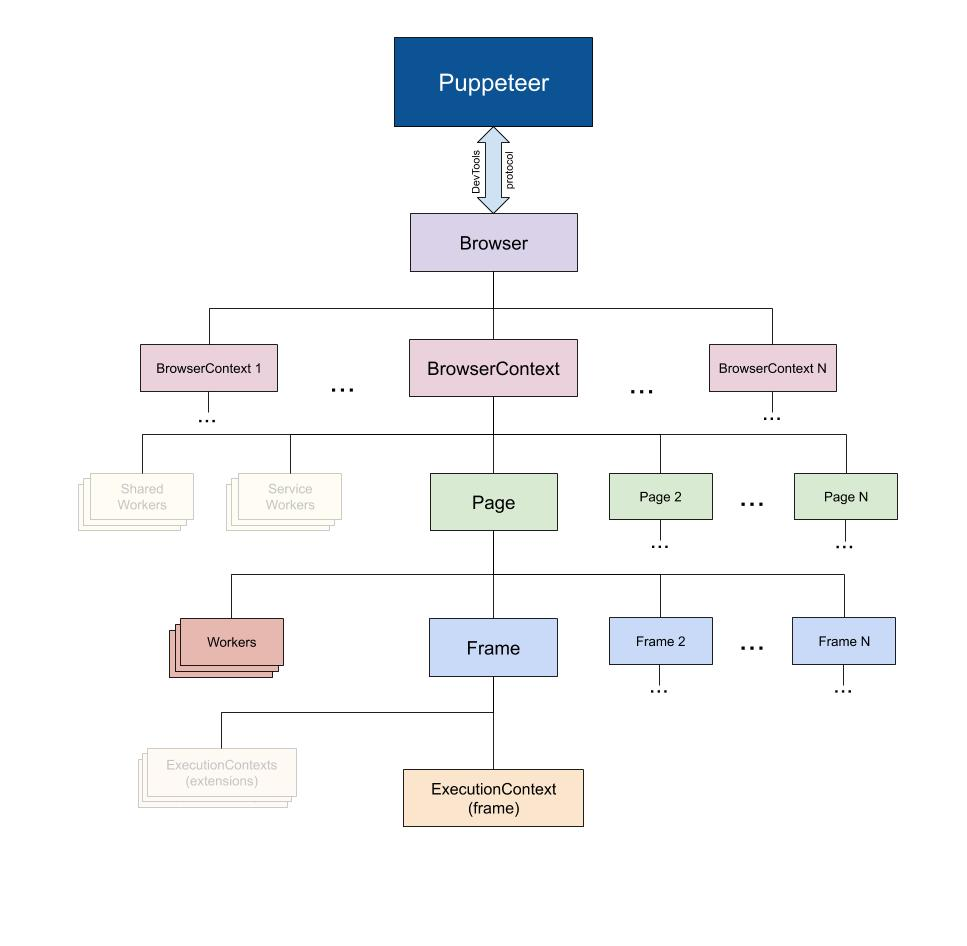
\includegraphics[width=9cm,height=10cm]{Images/C-2/puppeteeroverview.jpg}
				\caption{Struktur diagram \textit{Puppeteer}}
				\label{puppeteeroverview}
			\end{figure}
			
			\indent Pada tugas akhir ini, \textit{Puppeteer} akan digunakan sebagai alat untuk mengontrol \textit{Headless Browser} yang akan diimplementasikan pada sistem perangkat lunak yang akan dibangun, karena lebih mumpuni dan memiliki beragam fitur \textit{API} untuk mengakses \textit{Headless Chrome} dibandingkan dengan pustaka \textit{Node} yang lain.
		
	\section{\textit{Docker}}
		\textit{Docker} adalah sebuah platform terbuka yang berfungsi sebagai wadah untuk membangun, membungkus, dan menjalankan aplikasi supaya dapat berfungsi sebagaimana mestinya. \textit{Docker} memungkinkan untuk memisahkankan aplikasi dari infrastruktur supaya \textit{software} dapat di jalankan dengan lebih cepat. \textit{Docker} pada dasarnya memperluas \textit{LXC(Linux Containers)} menggunakan kernel dan \textit{API} pada level aplikasi yang akan dijalankan secara bersamaan pada isolasi \textit{CPU}, memori, I/O, jaringan dan yang lainnya. \textit{Docker} juga menggunakan \textit{namespaces} untuk mengisolasi segala tampilan pada aplikasi yang mendasari lingkungan operasinya, termasuk \textit{process tree}, jaringan, ID pengguna, dan file sistem. 
		
		\indent \textit{Docker Container} dibuat oleh sebuah \textit{Docker Images}. \textit{Docker Images} hanya mencakup dasar dari operasi sistem atau hanya memuat set dari \textit{prebuilt} aplikasi yang sudah siap dijalankan. Ketika membuat \textit{Docker Images}, bisa menjalankan perintah (yaitu apt-get install) membentuk lapisan baru diatas lapisan sebelumnya. Perintah tersebut bisa dijalankan manual satu-persatu atau secara otomatis menggunakan \textit{Dockerfile}. 
		
		\indent Setiap \textit{Dockerfile} adalah kombinasi beberapa perintah yang dibuat menjadi menjadi satu atau \textit{script} yang bisa dijalankan secara otomatis sebagai \textit{Docker Images} utama atau untuk membuat \textit{Docker Images} yang baru\cite{docker}\cite{docker_2}. \textit{Docker} juga menyediakan layanan untuk mengunduh dan mengupload \textit{Docker images} melalui \texttt{https://hub.docker.com/}. Untuk melihat perbedaan antara kontainer dan \textit{VM(Virtual Machine)} dapat dilihat pada Gambar \ref{containervm}.
	
		\indent Pada tugas akhir ini, \textit{Docker Container} akan digunakan sebagai pengguna untuk mengakses web yang akan diuji, dan bisa diumpamakan sebagai pengguna asli untuk otomasi pengujiannya. \\
		
		\begin{figure}[H]
			\centering
			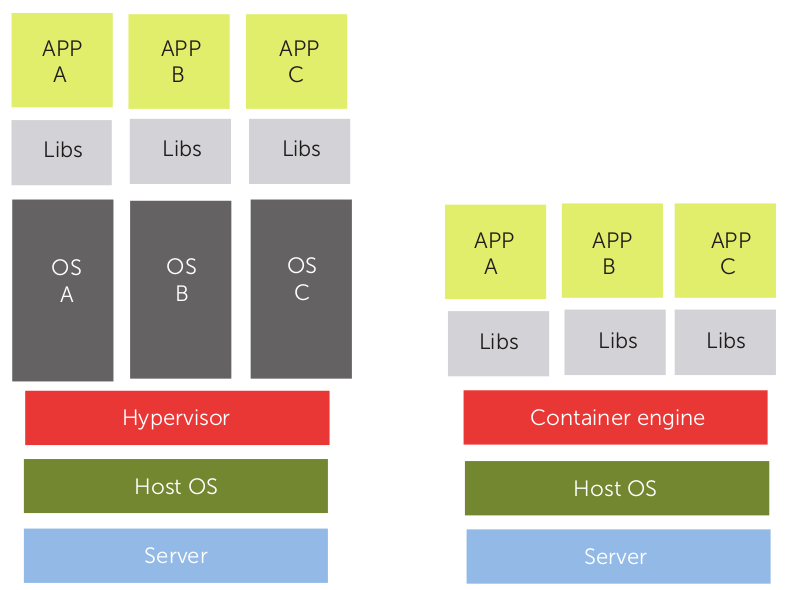
\includegraphics[width=9cm,height=7cm]{Images/C-2/containervm.png}
			\caption{Perbandingan kontainer dan \textit{Virtual Machine}\cite{docker_2}}
			\label{containervm}
		\end{figure}
	
		\subsection{\textit{Docker Swarm}}
			\textit{Docker Swarm} - disebut juga \textit{Swarm} adalah mode pada \textit{Docker} yang memiliki fitur yang tertanam pada mesinnya untuk Manajemen \textit{Cluster} atau \textit{Orkestrasi}. Pada mode \textit{Swarm} akan terdapat lebih dari satu \textit{host} dimana \textit{host} tersebut bisa berfungsi sebagai manager, worker, atau bisa juga keduanya. Konsep pada \textit{Swarm} antara lain adalah \textit{Nodes}, \textit{Services}, \textit{Tasks} dan \textit{Load Balancing}. Mode \textit{Swarm} juga memudahkan untuk mengatur bagian replikasi, jaringan, penyimpanan, port dan sebagainya.
			
			\indent Dibandingkan dengan kontainer yang berdiri sendiri, \textit{Swarm} lebih mudah untuk mengubah konfigurasi servis, termasuk penyimpanan dan jaringannya tanpa harus menyalakan kembali kontainer secara manual. \textit{Docker} akan otomatis memperbarui konfigurasi dengan cara menghentikan \textit{service task} yang memiliki konfigurasi lama, kemudian akan membuat kembali \textit{service task} menggunakan konfigurasi yang sudah diperbarui. \textit{Swarm} juga bisa menggunakan \textit{Docker Compose} untuk mendefinisikan dan menjalankan kontainer, \textit{Docker Compose} menggunakan \textit{YAML file} sebagai konfigurasinya.\cite{docker_swarm}.
			
			\indent Pada saat mode \textit{Swarm}, \textit{node manager} akan mengimplementasikan \textit{Raft Consensus Algorithm} untuk memanajemen \textit{cluster}. \textit{Consensus} memungkinan manajer untuk mengatur dan menjadwal \textit{tasks} pada setiap \textit{cluster} dan memastikan status tetap konsisten, dimana ketika ada salah satu \textit{nodes} yang gagal dalam mejalankan servis, manajer bisa mengembalikan servis menjadi stabil kembali\cite{docker_swarm_raft}. Untuk melihat rute diagram ketika mode \textit{Swarm} dapat dilihat pada Gambar \ref{swarmdiagramroute}.
			
			\begin{figure}[H]
				\centering
				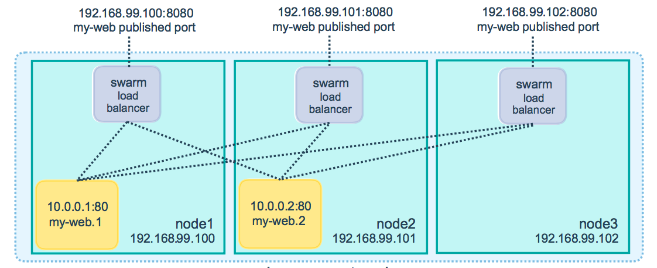
\includegraphics[width=10cm,height=4cm]{Images/C-2/swarmdiagramroute.png}
				\caption{Rute diagram ketika mode \textit{Swarm}\cite{docker_swarm_route}}
				\label{swarmdiagramroute}
			\end{figure}
		
			\indent Pada tugas akhir ini, \textit{Docker Swarm} akan digunakan sebagai manager atau okestrasi yang mengatur segala servis maupun aktivitas \textit{Docker Container} dan sebagai \textit{Load Balancer} untuk pembagian beban kontainer pada setiap \textit{nodes} yang merupakan instansi dari \textit{Docker Swarm} tersebut.
			
			
		
	\section{\textit{Laravel}}
		\textit{Laravel} adalah salah satu kerangka kerja yang berbahasa \textit{PHP} dan dibuat untuk memudahkan pengembang untuk mengembangan dan mendesain sebuah web yang menekankan kesederhanaan dan fleksibitas. Kerangka kerja ini mendukung metode \textit{MVC(Model-View-Controller)}. dimana \textit{MVC} digunakan untuk mengembangkan sebuah aplikasi yang memisahkan data(\textit{Model}) dari tampilan(\textit{View}) dan juga dari logika dari aplikasi tersebut(\textit{Controller})\cite{laraveframework}.
		
		\indent \textit{Model} digunakan untuk memanipulasi data dari basis data, \textit{View} berhubungan dengan antarmuka web seperti \textit{HTML}, \textit{CSS} dan \textit{JS} sebagai data pada pengguna. \textit{Controller} berhubungan dengan segala urusan logika pada servis web tersebut atau juga bisa disebut otaknya. \textit{Controller} juga berfungsi sebagai jembatan antara \textit{View} dan \textit{Model}\cite{laraveframework}.
	
		\indent Pada tugas akhir ini, kerangka kerja \textit{Laravel} akan digunakan untuk mengimplementasikan aplikasi web yang dibangun pada tugas akhir ini, dimana kerangka kerja ini sangat banyak digunakan oleh pengembang, memiliki dokumentasi resmi yang sangat baik, serta forum yang cukup baik. \textit{Laravel} yang akan digunakan adalah versi 5.8.
		
	\section{\textit{Python}}
		\textit{Python} adalah bahasa pemrograman tingkat tinggi yang didukung oleh struktur data \textit{built-in} semantik dinamis, selain itu Python mendukung pemrograman \textit{procedural}, \textit{object-oriented} dan \textit{functional}. \textit{Python} merupakan bahasa pemrograman \textit{interpreted}, oleh sebab itu, \textit{Python} tidak memakan biaya untuk kompilasi, sehingga proses pengembangan, pengujian dan \textit{debug} menjadi lebih cepat.
		 
		\indent Kelebihan bahasa pemrograman ini adalah memiliki modul dan \textit{package}, serta memiliki banyak standar pustaka yang didistribusikan secara bebas dan gratis. Selain itu \textit{Python} mudah dibaca karena memiliki sintaksis yang sederhana, sehingga dapat mengurangi biaya \textit{maintenance}. \textit{Debug} pada \textit{Python} juga mudah karena tidak akan terjadi \textit{segmentation fault}, namun akan memberi umpan balik berupa \textit{exception} apabila terdapat kesalahan atau \textit{error}\cite{python}.
		
		\indent Pada tugas akhir ini, Bahasa pemrograman \textit{Python} akan digunakan untuk mengimplementasikan algoritme \textit{task queue} pada sistem yang akan dibangun. \textit{Python} yang digunakan adalah versi 3.6.8.